% questions.tex —— 2010 年·普通高等学校招生考试·陕西卷·理科 · 题目内容片段（无答案）
% 由 tools/generate_projects.py 依来源总账自 2010/2010_数学真题_陕西理_试题.md 生成，勿手改（改源 MD 后重跑）
状态：needs-review；依固定候选 PDF 两页（印刷页 623–624）逐题核验，八幅图已矢量重绘。原页未印分值，不补。
原页第 15 题以「15．三选一．」起，下分【A】【B】【C】三小题（不等式选讲、几何证明选讲、坐标系与参数方程），属选修模块选考，三选一；此栏目名照录，不改。
\gkpart{一、选择题}
\begin{question}
\gkti{1}集合 $A=\{x\mid -1\leqslant x\leqslant 2\}$，$B=\{x\mid x<1\}$，则 $A\cap(\complement_{\mathbf R}B)=$（　）

（A）$\{x\mid x>1\}$

（B）$\{x\mid x\geqslant 1\}$

（C）$\{x\mid 1<x\leqslant 2\}$

（D）$\{x\mid 1\leqslant x\leqslant 2\}$

\end{question}
\begin{question}
\gkti{2}复数 $z=\dfrac{\mathrm i}{1+\mathrm i}$ 在复平面上对应的点位于（　）

（A）第一象限

（B）第二象限

（C）第三象限

（D）第四象限

\end{question}
\begin{question}
\gkti{3}对于函数 $f(x)=2\sin x\cos x$，下列选项中正确的是（　）

（A）对于 $f(x)$ 在 $\left(\dfrac{\pi}{4},\dfrac{\pi}{2}\right)$ 上是递增的

（B）$f(x)$ 的图象关于原点对称

（C）$f(x)$ 的最小正周期为 $2\pi$

（D）$f(x)$ 的最大值为 $2$

\end{question}
\begin{question}
\gkti{4}$\left(x+\dfrac{a}{x}\right)^5$（$x\in\mathbf R$）展开式中 $x^3$ 的系数为 $10$，则实数 $a$ 等于（　）

（A）$-1$

（B）$\dfrac12$

（C）$1$

（D）$2$

\end{question}
\begin{question}
\gkti{5}已知函数 $f(x)=\begin{cases}2^x+1,&x<1,\\[2pt]x^2+ax,&x\geqslant 1,\end{cases}$ 若 $f(f(0))=4a$，则实数 $a$ 等于（　）

（A）$\dfrac12$

（B）$\dfrac45$

（C）$2$

（D）$9$

\Needspace{0.4\textheight}
\end{question}
\begingroup
\renewenvironment{question}{\Needspace{0.5\textheight}}{}
\begin{question}
\gkti{6}如图所示的求样本 $x_1$，$x_2$，$\cdots$，$x_{10}$ 平均数 $\bar x$ 的程序框图，图中空白框中应填入的内容为（　）

（A）$S=S+x_n$

（B）$S=S+\dfrac{x_n}{n}$

（C）$S=S+n$

（D）$S=S+\dfrac1n$
\nopagebreak[4]
\begin{center}% 2010 年陕西卷理科第 6 题：求样本平均数的程序框图。
% 来源 PDF：普通高考/2010/2010陕西理.pdf，SHA-256 8406e303e7aa1ac7813893781c903a7d9c904530028e6fd1c06062d1c32bd645。
% 原页：第 1 页（A3 三栏）第 1 栏下部，书页码 623。
% 重绘依据：照原页——竖排主干为 开始→输入 x1,…,x10→n=1,S=0→〔空白框〕→判断 n≥10?
%   →「是」向下进 x̄=S/n→输出 x̄→结束；「否」向左进 n=n+1 框，该框顶部再向上折回主干，
%   在空白框正上方汇入主干（原页此处只画一个向下箭头进入空白框）。空白框在原页为空。
\begin{tikzpicture}[semithick,
  every node/.style={inner sep=2pt},
  box/.style={draw, minimum width=3.5cm, minimum height=0.66cm, align=center},
  round/.style={draw, rounded corners=7pt, minimum width=1.7cm,
    minimum height=0.66cm, align=center},
  para/.style={draw, trapezium, trapezium left angle=72, trapezium right angle=108,
    minimum width=6.1cm, minimum height=0.74cm, align=center},
  dec/.style={draw, diamond, aspect=2.7, minimum width=2.9cm,
    minimum height=1.05cm, align=center},
  arr/.style={->, >=stealth}]

  \node[round] (start) at (0,0) {开始};
  \node[para]  (in)    at (0,-1.20) {输入 $x_1,\,x_2,\,\cdots,\,x_{10}$};
  \node[box]   (init)  at (0,-2.45) {$n=1$，$S=0$};
  \node[box, minimum height=0.86cm] (acc) at (0,-3.80) {};
  \node[dec]   (test)  at (0,-5.60) {$n\geqslant 10$};
  \node[box]   (inc)   at (-4.55,-3.80) {$n=n+1$};
  \node[box, minimum height=1.50cm, text height=0.72cm, text depth=0.62cm] (avg) at (0,-7.45) {$\bar x=\dfrac{S}{n}$};
  \node[para]  (out)   at (0,-9.55) {输出 $\bar x$};
  \node[round] (end)   at (0,-11.20) {结束};

  \draw[arr] (start) -- (in);
  \draw[arr] (in) -- (init);
  \draw[arr] (init) -- (acc);

  \draw[arr] (acc) -- (test);
  \draw[arr] (test) -- (avg);
  \node[right] at (0.16,-6.40) {是};
  \draw[arr] (avg) -- (out);
  \draw[arr] (out) -- (end);

  % 「否」分支：由判断框左顶点向左，再向上进入 n=n+1 框
  \draw[arr] (test.west) -- (-4.55,-5.60) -- (inc.south);
  \node[above] at (-2.55,-5.45) {否};

  % 回边：n=n+1 框顶部向上、再向右，汇入空白框上方的竖线
  \draw (inc.north) -- (-4.55,-2.95) -- (0,-2.95);
\end{tikzpicture}
\end{center}
\nopagebreak[4]
\Needspace{0.4\textheight}
\end{question}
\endgroup
\begingroup
\renewenvironment{question}{\Needspace{0.5\textheight}}{}
\begin{question}
\gkti{7}若某空间几何体的三视图如图所示，则该几何体的体积是（　）

（A）$\dfrac13$

（B）$\dfrac23$

（C）$1$

（D）$2$
\nopagebreak[4]
\begin{center}% 2010 年陕西卷理科第 7 题：某空间几何体的三视图。
% 来源 PDF：普通高考/2010/2010陕西理.pdf，SHA-256 8406e303e7aa1ac7813893781c903a7d9c904530028e6fd1c06062d1c32bd645。
% 原页：第 1 页（A3 三栏）第 2 栏上部，书页码 623。
% 重绘依据：照原页——上方为矩形主视图（宽标 √2、高标 1），其右上角右侧另有直角三角形左视图
%   （竖直边在左、斜边自左上落向右下、底边水平），下方为正方形俯视图（右边标 √2）。
%   三个视图按原页的上下、左右相对位置摆放；尺寸线用细线加双向箭头，标注照录。
\begin{tikzpicture}[semithick, x=1cm, y=1cm,
  dim/.style={<->, >=stealth, thin},
  ext/.style={thin}]

  % 主视图：宽 √2≈1.90，高 1≈1.34
  \draw (0,2.60) rectangle (1.90,3.94);
  \node at (0.95,2.35) {主视图};

  % 俯视图：边长 1.90 的正方形
  \draw (0,-0.20) rectangle (1.90,1.70);
  \node at (0.95,-0.45) {俯视图};

  % 主视图宽度尺寸线（√2）
  \draw[ext] (0,3.94) -- (0,4.32);
  \draw[ext] (1.90,3.94) -- (1.90,4.32);
  \draw[dim] (0,4.18) -- (1.90,4.18);
  \node[above] at (0.95,4.18) {$\sqrt2$};

  % 主视图高度尺寸线（1）
  \draw[ext] (1.90,2.60) -- (2.26,2.60);
  \draw[ext] (1.90,3.94) -- (2.26,3.94);
  \draw[dim] (2.12,2.60) -- (2.12,3.94);
  \node[right] at (2.28,3.27) {$1$};

  % 俯视图高度尺寸线（√2）
  \draw[ext] (1.90,-0.20) -- (2.26,-0.20);
  \draw[ext] (1.90,1.70) -- (2.26,1.70);
  \draw[dim] (2.12,-0.20) -- (2.12,1.70);
  \node[right] at (2.28,0.75) {$\sqrt2$};

  % 左视图：直角三角形，竖直直角边在左，斜边自左上落向右下
  \draw (3.60,2.60) -- (3.60,3.94) -- (5.50,2.60) -- cycle;
  \node at (4.55,2.35) {左视图};
\end{tikzpicture}
\end{center}
\nopagebreak[4]
\end{question}
\endgroup
\begin{question}
\gkti{8}已知抛物线 $y^2=2px$（$p>0$）的准线与圆 $x^2+y^2-6x-7=0$ 相切，则 $p$ 的值为（　）

（A）$\dfrac12$

（B）$1$

（C）$2$

（D）$4$

\end{question}
\begin{question}
\gkti{9}对于数列 $\{a_n\}$，“$a_{n+1}>|a_n|$（$n=1$，$2$，$\cdots$）”是“$\{a_n\}$ 为递增数列”的（　）

（A）必要不充分条件

（B）充分不必要条件

（C）充要条件

（D）既不充分也不必要条件

\end{question}
\begin{question}
\gkti{10}某学校要召开学生代表大会，规定各班每 $10$ 人推选一名代表，当各班人数除以 $10$ 的余数大于 $6$ 时再增选一名代表．那么，各班可推选代表人数 $y$ 与该班人数 $x$ 之间的函数关系用取整函数 $y=[x]$（$[x]$ 表示不大于 $x$ 的最大整数）可以表示为（　）

（A）$y=\left[\dfrac{x}{10}\right]$

（B）$y=\left[\dfrac{x+3}{10}\right]$

（C）$y=\left[\dfrac{x+4}{10}\right]$

（D）$y=\left[\dfrac{x+5}{10}\right]$

\end{question}
\gkpart{二、填空题}
\begin{question}
\gkti{11}已知向量 $\boldsymbol a=(2,-1)$，$\boldsymbol b=(-1,m)$，$\boldsymbol c=(-1,2)$，若 $(\boldsymbol a+\boldsymbol b)\parallel\boldsymbol c$，则 $m=\underline{\qquad}$．

\end{question}
\begin{question}
\gkti{12}观察下列等式：$1^3+2^3=3^2$，$1^3+2^3+3^3=6^2$，$1^3+2^3+3^3+4^3=10^2$，$\cdots$，根据上述规律，第五个等式为 $\underline{\qquad}$．

\Needspace{0.4\textheight}
\end{question}
\begingroup
\renewenvironment{question}{\Needspace{0.5\textheight}}{}
\begin{question}
\gkti{13}从如图所示的长方形区域内任取一个点 $M(x,y)$，则点 $M$ 取自阴影部分的概率为 $\underline{\qquad}$．
\nopagebreak[4]
\begin{center}% 2010 年陕西卷理科第 13 题：长方形区域内的阴影部分（y=3x²、x=1 与 x 轴围成）。
% 来源 PDF：普通高考/2010/2010陕西理.pdf，SHA-256 8406e303e7aa1ac7813893781c903a7d9c904530028e6fd1c06062d1c32bd645。
% 原页：第 1 页（A3 三栏）第 2 栏中部，书页码 623。
% 重绘依据：照原页——坐标系中抛物线 y=3x² 自原点升到 (1,3)；y=3 处有一条水平线自 y 轴到 (1,3)，
%   x=1 处有一条竖直线自 x 轴到 (1,3)，二者与坐标轴围成长方形；阴影落在曲线与竖直线 x=1 之间、
%   即曲线下方贴 x 轴的那一块（曲线上方/左侧为空白）。曲线在 (1,3) 之外略向上延伸。
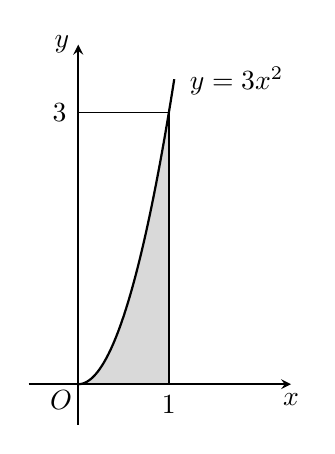
\begin{tikzpicture}[x=1.15cm, y=1.15cm, semithick, line join=round]

  % 阴影：曲线下方、x=1 左侧、x 轴上方
  \fill[gray!30] plot[domain=0:1, samples=60] (\x,{3*\x*\x}) -- (1,0) -- cycle;

  % 坐标轴
  \draw[->, >=stealth] (-0.55,0) -- (2.35,0) node[below, inner sep=3pt] {$x$};
  \draw[->, >=stealth] (0,-0.45) -- (0,3.75) node[left, inner sep=3pt] {$y$};

  % 长方形：y=3 的水平边、x=1 的竖直边
  \draw (0,3) -- (1,3);
  \draw (1,0) -- (1,3);

  % 抛物线 y=3x²（在 (1,3) 之外略向上延伸）
  \draw[thick, domain=0:1.06, samples=80] plot (\x,{3*\x*\x});
  \node[right] at (1.12,3.35) {$y=3x^2$};

  % 刻度与原点
  \node[below left, inner sep=2pt] at (0,0) {$O$};
  \node[below, inner sep=4pt] at (1,0) {$1$};
  \node[left, inner sep=4pt] at (0,3) {$3$};
\end{tikzpicture}
\end{center}
\nopagebreak[4]
\end{question}
\endgroup
\begin{question}
\gkti{14}铁矿石 $A$ 和 $B$ 的含铁率 $a$，冶炼每万吨铁矿石的 $\mathrm{CO_2}$ 排放量 $b$ 及每万吨铁矿石的价格 $c$ 如下表：

\begin{center}
\begin{tabular}{lrrr}
\toprule
 & $a$ & $b$（万吨） & $c$（百万元） \\
\midrule
$A$ & $50\%$ & $1$ & $3$ \\
$B$ & $70\%$ & $0.5$ & $6$ \\
\bottomrule
\end{tabular}
\end{center}

某冶炼厂至少要生产 $1.9$（万吨）铁，若要求 $\mathrm{CO_2}$ 的排放量不超过 $2$（万吨），则购买铁矿石的最少费用为 $\underline{\qquad}$（百万元）．

\Needspace{0.4\textheight}
\end{question}
\begingroup
\renewenvironment{question}{\Needspace{0.35\textheight}}{}
\begin{question}
\gkti{15}三选一．

【A】不等式 $|x+3|-|x-2|\geqslant 3$ 的解集为 $\underline{\qquad}$．

【B】如图，已知 $\mathrm{Rt}\triangle ABC$ 的两条直角边 $AC$，$BC$ 的长分别为 $3\ \mathrm{cm}$，$4\ \mathrm{cm}$，以 $AC$ 为直径的圆与 $AB$ 交于点 $D$，则 $\dfrac{BD}{DA}=$ $\underline{\qquad}$．
\nopagebreak[4]
\begin{center}% 2010 年陕西卷理科第 15 题【B】：Rt△ABC 与以 AC 为直径的圆。
% 来源 PDF：普通高考/2010/2010陕西理.pdf，SHA-256 8406e303e7aa1ac7813893781c903a7d9c904530028e6fd1c06062d1c32bd645。
% 原页：第 1 页（A3 三栏）第 3 栏上部，书页码 623。
% 重绘依据：照原页——A 在最高处，C 在其正下方（直角顶点，直角符号朝内），B 在左下方；
%   圆以 AC 为直径（圆心 O 标出圆点），圆周向右鼓出 AC 之外；斜边 AB 与圆交于 D（D 在 A 与 B 之间）。
%   按题设 AC=3、BC=4 取坐标：C=(0,0)，A=(0,3)，B=(-4,0)，则 D=(-1.44,1.92)。
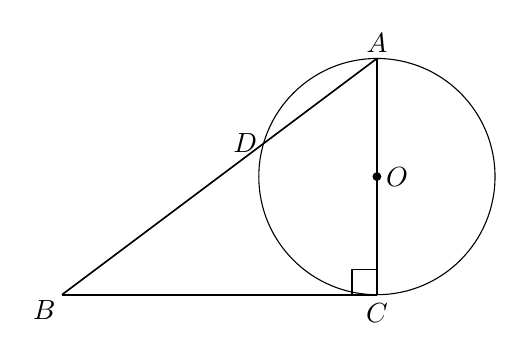
\begin{tikzpicture}[semithick, line join=round]
  \coordinate (C) at (0,0);
  \coordinate (A) at (0,3);
  \coordinate (B) at (-4,0);
  \coordinate (O) at (0,1.5);
  \coordinate (D) at (-1.44,1.92);

  % 以 AC 为直径的圆
  \draw[thin] (O) circle (1.5);

  % 三角形三边
  \draw (A) -- (B);
  \draw (B) -- (C);
  \draw (C) -- (A);

  % C 处直角符号
  \draw (0,0.32) -- (-0.32,0.32) -- (-0.32,0);

  % 圆心
  \fill (O) circle (1.6pt);

  % 顶点与交点标注
  \node[above, inner sep=2pt] at (A) {$A$};
  \node[below left, inner sep=2pt] at (B) {$B$};
  \node[below, inner sep=3pt] at (C) {$C$};
  \node[right, inner sep=3pt] at (O) {$O$};
  \node[left, inner sep=2pt] at (D) {$D$};
\end{tikzpicture}
\end{center}
\nopagebreak[4]
【C】已知圆 $C$ 的参数方程为 $\begin{cases}x=\cos\alpha,\\[2pt]y=1+\sin\alpha,\end{cases}$（$\alpha$ 为参数），以原点为极点，$x$ 轴正半轴为极轴建立极坐标系，直线 $l$ 的极坐标方程为 $\rho\sin\theta=1$，则直线 $l$ 与圆 $C$ 的交点的直角坐标为 $\underline{\qquad}$．

\end{question}
\endgroup
\gkpart{三、解答题}
\begin{question}
\gkti{16}已知 $\{a_n\}$ 是公差不为零的等差数列，$a_1=1$ 且 $a_1$，$a_3$，$a_9$ 成等比数列．

（1）求数列 $\{a_n\}$ 的通项；

（2）求数列 $\{2^{a_n}\}$ 的前 $n$ 项和 $S_n$．

\Needspace{0.4\textheight}
\end{question}
\begingroup
\renewenvironment{question}{\Needspace{0.5\textheight}}{}
\begin{question}
\gkti{17}如图，$A$，$B$ 是海面上位于东西方向相距 $5(3+\sqrt3)$ 海里的两个观测点．现位于 $A$ 点北偏东 $45^\circ$，$B$ 点北偏西 $60^\circ$ 的 $D$ 点有一艘轮船发出求救信号，位于 $B$ 点南偏西 $60^\circ$ 且与 $B$ 点相距 $20\sqrt3$ 海里的 $C$ 点的救援船立即前往营救，其航行速度为 $30$ 海里/小时，该救援船到达 $D$ 点需要多长时间？
\nopagebreak[4]
\begin{center}% 2010 年陕西卷理科第 17 题：海面上的两个观测点 A、B 与船 D、救援船 C 的方位图。
% 来源 PDF：普通高考/2010/2010陕西理.pdf，SHA-256 8406e303e7aa1ac7813893781c903a7d9c904530028e6fd1c06062d1c32bd645。
% 原页：第 1 页（A3 三栏）第 3 栏下部，书页码 623。
% 重绘依据：照原页——A 在左、B 在右，AB 为水平（东西方向）；A、B 上方各有一条竖直「北」向箭头；
%   D 在 AB 上方偏左，DA、DB 均连；45° 标在 A 的北向射线与 AD 之间，60° 标在 B 的北向射线与 BD 之间，
%   另一 60° 标在 B 的南向射线（北向线的延长线）与 BC 之间；C 在 A 的左下方，CA、CB 均连。
%   按题设取 AB=5(3+√3) 的比例坐标（整体缩放 1/4）：A=(0,0)，B=(5.90,0)，D=(2.17,2.17)，C=(-1.58,-4.33)。
\begin{tikzpicture}[semithick, line join=round]
  \coordinate (A) at (0,0);
  \coordinate (B) at (5.90,0);
  \coordinate (D) at (2.17,2.17);
  \coordinate (C) at (-1.58,-4.33);

  % 方位线：AB 水平；DA、DB；CA、CB
  \draw (A) -- (B);
  \draw (D) -- (A);
  \draw (D) -- (B);
  \draw (C) -- (A);
  \draw (C) -- (B);

  % A 处的北向箭头
  \draw[->, >=stealth] (0,0) -- (0,3.05);
  \node[above, inner sep=2pt] at (0,3.05) {北};

  % B 处的竖直方位线（上端带箭头，下端延伸以标示南向）
  \draw[->, >=stealth] (5.90,-1.35) -- (5.90,3.05);
  \node[above, inner sep=2pt] at (5.90,3.05) {北};

  % 角标记与度数
  \draw (45:0.80) arc[start angle=45, end angle=90, radius=0.80];
  \node at (67:1.30) {$45^\circ$};

  \draw (5.90,0) ++(90:1.00) arc[start angle=90, end angle=150, radius=1.00];
  \node at ($(5.90,0)+(118:1.55)$) {$60^\circ$};

  \draw (5.90,0) ++(210:1.00) arc[start angle=210, end angle=270, radius=1.00];
  \node at ($(5.90,0)+(238:1.50)$) {$60^\circ$};

  % 顶点标注
  \node[left, inner sep=3pt] at (A) {$A$};
  \node[right, inner sep=3pt] at (B) {$B$};
  \node[above, inner sep=2pt] at (D) {$D$};
  \node[left, inner sep=3pt] at (C) {$C$};
\end{tikzpicture}
\end{center}
\nopagebreak[4]
\Needspace{0.4\textheight}
\end{question}
\endgroup
\begingroup
\renewenvironment{question}{\Needspace{0.5\textheight}}{}
\begin{question}
\gkti{18}如图，在四棱锥 $P-ABCD$ 中，底面 $ABCD$ 是矩形，$PA\perp$ 平面 $ABCD$，$AP=AB=2$，$BC=2\sqrt2$，$E$，$F$ 分别是 $AD$，$PC$ 的中点．

（1）证明：$PC\perp$ 平面 $BEF$；

（2）求平面 $BEF$ 与平面 $BAP$ 夹角的大小．
\nopagebreak[4]
\begin{center}% 2010 年陕西卷理科第 18 题：四棱锥 P-ABCD 与平面 BEF。
% 来源 PDF：普通高考/2010/2010陕西理.pdf，SHA-256 8406e303e7aa1ac7813893781c903a7d9c904530028e6fd1c06062d1c32bd645。
% 原页：第 2 页（A3 三栏）第 1 栏上部，书页码 624。
% 重绘依据：照原页——P 在最高处、A 在其下方（A 为被遮挡的后角，故 PA 画虚线），
%   B 在左下、C 在右下、D 在右侧与 A 同一水平高度；矩形 ABCD 中 AB、AD 为被遮挡的边（虚线），
%   BC、CD 为可见边（实线）；PB、PC、PD 为可见棱（实线）。
%   E 为 AD 中点、F 为 PC 中点：BF 落在可见侧面 PBC 内（实线），BE、EF 为体内辅助线（虚线）。
%   坐标（cm）：B=(0,0)，C=(6.4,0)，A=(1.9,2.3)，D=(8.3,2.3)，P=(2.0,7.6)，
%   则 E=(5.1,2.3)，F=(4.2,3.8)。
\begin{tikzpicture}[semithick, line join=round]
  \coordinate (B) at (0,0);
  \coordinate (C) at (6.4,0);
  \coordinate (A) at (1.9,2.3);
  \coordinate (D) at (8.3,2.3);
  \coordinate (P) at (2.0,7.6);
  \coordinate (E) at (5.1,2.3);
  \coordinate (F) at (4.2,3.8);

  % 可见棱与可见底边（实线）
  \draw (P) -- (B);
  \draw (P) -- (C);
  \draw (P) -- (D);
  \draw (B) -- (C);
  \draw (C) -- (D);
  \draw (B) -- (F);

  % 被遮挡的棱与体内辅助线（虚线）
  \draw[dashed] (P) -- (A);
  \draw[dashed] (A) -- (B);
  \draw[dashed] (A) -- (D);
  \draw[dashed] (B) -- (E);
  \draw[dashed] (E) -- (F);

  % 中点记号
  \draw ($(E)!0.055cm!90:(A)$) -- ($(E)!-0.055cm!90:(A)$);
  \draw ($(F)!0.055cm!90:(P)$) -- ($(F)!-0.055cm!90:(P)$);

  % 顶点标注
  \node[above, inner sep=2pt] at (P) {$P$};
  \node[above left, inner sep=1pt] at (A) {$A$};
  \node[below left, inner sep=2pt] at (B) {$B$};
  \node[below right, inner sep=2pt] at (C) {$C$};
  \node[right, inner sep=3pt] at (D) {$D$};
  \node[below, inner sep=3pt] at (E) {$E$};
  \node[right, inner sep=3pt] at (F) {$F$};
\end{tikzpicture}
\end{center}
\nopagebreak[4]
\Needspace{0.4\textheight}
\end{question}
\endgroup
\begingroup
\renewenvironment{question}{\Needspace{0.5\textheight}}{}
\begin{question}
\gkti{19}为了解学生身高情况，某校以 $10\%$ 的比例对全校 $700$ 名学生按性别进行分层抽样调查，测得身高情况的统计图如下：

（1）估计该校男生的人数；

（2）估计该校学生身高在 $170\sim 185\ \mathrm{cm}$ 之间的概率；

（3）从样本中身高在 $165\sim 180\ \mathrm{cm}$ 之间的女生中任选 $2$ 人，求至少有 $1$ 人身高在 $170\sim 180\ \mathrm{cm}$ 之间的概率．
\nopagebreak[4]
\begin{center}% 2010 年陕西卷理科第 19 题：男、女生身高频数分布直方图（样本各 40 人、30 人）。
% 来源 PDF：普通高考/2010/2010陕西理.pdf，SHA-256 8406e303e7aa1ac7813893781c903a7d9c904530028e6fd1c06062d1c32bd645。
% 原页：第 2 页（A3 三栏）第 1 栏下部，书页码 624。
% 重绘依据：照原页——左「男生」、右「女生」两幅频数直方图，横轴 身高/cm 自 160 起每 5 cm 一组
%   至 190，纵轴为频数（原点处画有断裂符号）。
%   男生各组频数依次为 2, 5, 14, 13, 4, 2（合计 40）；女生依次为 1, 7, 12, 6, 3, 1（合计 30）。
%   原页在各组上沿引出水平虚线并标注频数：男生 14、13、5、4、2；女生 12、7、6、3、1。
\begin{tikzpicture}[x=0.62cm, y=0.30cm, semithick, line join=round,
  lbl/.style={font=\scriptsize, inner sep=1pt}]

  % ================= 男生 =================
  \begin{scope}
    % 坐标轴
    \draw[->, >=stealth] (-0.55,-1.20) -- (-0.55,16.00);
    \draw[->, >=stealth] (-1.20,0) -- (7.05,0);
    \node[lbl, right] at (-0.60,14.75) {频数};
    \node[lbl, above] at (6.40,1.00) {身高/cm};

    % 原点断裂符号
    \draw[thin] (-0.98,0) -- (-0.90,1.10) -- (-0.82,-1.10) -- (-0.74,1.10) -- (-0.66,0);
    \node[lbl, below] at (-1.02,-0.20) {$0$};

    % 各组矩形
    \foreach \i/\h in {0/2, 1/5, 2/14, 3/13, 4/4, 5/2} {
      \draw (\i,0) rectangle (\i+1,\h);
    }

    % 频数虚线（自纵轴引到该频数组的左沿）
    \foreach \i/\h in {0/2, 1/5, 2/14, 3/13, 4/4} {
      \draw[thin, dashed] (-0.55,\h) -- (\i,\h);
    }
    \node[lbl, left] at (-0.62,2) {$2$};
    \node[lbl, left] at (-0.62,5) {$5$};
    \node[lbl, left] at (-0.62,4) {$4$};
    \node[lbl, left] at (-0.62,14) {$14$};
    \node[lbl, left] at (-0.62,13) {$13$};

    % 横轴刻度
    \foreach \i/\v in {0/160, 1/165, 2/170, 3/175, 4/180, 5/185, 6/190} {
      \draw[thin] (\i,0) -- (\i,-0.90);
      \node[lbl, below] at (\i,-1.05) {\v};
    }

    % 标题
    \node at (3.0,17.30) {男生};
  \end{scope}

  % ================= 女生 =================
  \begin{scope}[xshift=5.35cm]
    \draw[->, >=stealth] (-0.55,-1.20) -- (-0.55,16.00);
    \draw[->, >=stealth] (-1.20,0) -- (7.05,0);
    \node[lbl, right] at (-0.60,14.75) {频数};
    \node[lbl, above] at (6.40,1.00) {身高/cm};

    \draw[thin] (-0.98,0) -- (-0.90,1.10) -- (-0.82,-1.10) -- (-0.74,1.10) -- (-0.66,0);
    \node[lbl, below] at (-1.02,-0.20) {$0$};

    \foreach \i/\h in {0/1, 1/7, 2/12, 3/6, 4/3, 5/1} {
      \draw (\i,0) rectangle (\i+1,\h);
    }

    \foreach \i/\h in {0/1, 1/7, 2/12, 3/6, 4/3} {
      \draw[thin, dashed] (-0.55,\h) -- (\i,\h);
    }
    \node[lbl, left] at (-0.62,1) {$1$};
    \node[lbl, left] at (-0.62,7) {$7$};
    \node[lbl, left] at (-0.62,6) {$6$};
    \node[lbl, left] at (-0.62,12) {$12$};
    \node[lbl, left] at (-0.62,3) {$3$};

    \foreach \i/\v in {0/160, 1/165, 2/170, 3/175, 4/180, 5/185, 6/190} {
      \draw[thin] (\i,0) -- (\i,-0.90);
      \node[lbl, below] at (\i,-1.05) {\v};
    }

    \node at (3.0,17.30) {女生};
  \end{scope}
\end{tikzpicture}
\end{center}
\nopagebreak[4]
\Needspace{0.4\textheight}
\end{question}
\endgroup
\begingroup
\renewenvironment{question}{\Needspace{0.5\textheight}}{}
\begin{question}
\gkti{20}如图，椭圆 $C:\dfrac{x^2}{a^2}+\dfrac{y^2}{b^2}=1$ 的顶点为 $A_1$，$A_2$，$B_1$，$B_2$，焦点为 $F_1$，$F_2$，$|A_1B_1|=\sqrt7$，$S_{\square A_1B_1A_2B_2}=2S_{\square B_1F_1B_2F_2}$．

（1）求椭圆 $C$ 的方程；

（2）设 $n$ 是过原点的直线，$l$ 是与 $n$ 垂直相交于 $P$ 点、与椭圆相交于 $A$，$B$ 两点的直线，$|\overrightarrow{OP}|=1$．是否存在上述直线 $l$ 使 $\overrightarrow{AP}\cdot\overrightarrow{PB}=1$ 成立？若存在，求出直线 $l$ 的方程；若不存在，请说明理由．
\nopagebreak[4]
\begin{center}% 2010 年陕西卷理科第 20 题：椭圆 C 与过原点直线 n、与之垂直的直线 l。
% 来源 PDF：普通高考/2010/2010陕西理.pdf，SHA-256 8406e303e7aa1ac7813893781c903a7d9c904530028e6fd1c06062d1c32bd645。
% 原页：第 2 页（A3 三栏）第 2 栏上部，书页码 624。
% 重绘依据：照原页——椭圆中心为 O，长短轴端点为 A1（左）、A2（右）、B1（上）、B2（下），
%   两焦点 F1（左）、F2（右）用圆点标出；直线 n 过 O 斜向右上到 P，直线 l 过 P 且与 n 垂直，
%   在 P 处画直角符号；l 与椭圆交于右上的 A、右下的 B，并在 A、B 之外略作延长。
%   按 (1) 的结论 a=2、b=√3 取图（整体乘 1.5）：A1=(-3,0)，A2=(3,0)，B1=(0,2.598)，B2=(0,-2.598)，
%   F1=(-1.5,0)，F2=(1.5,0)；再取 |OP|=1.5、n 的倾角约 18.4°，得 P=(1.423,0.474)，
%   l: y=-3x+4.743，与椭圆交于 A=(0.742,2.517)、B=(2.177,-1.788)。
\begin{tikzpicture}[semithick, line join=round]
  \coordinate (O)  at (0,0);
  \coordinate (A1) at (-3,0);
  \coordinate (A2) at (3,0);
  \coordinate (B1) at (0,{1.5*sqrt(3)});
  \coordinate (B2) at (0,{-1.5*sqrt(3)});
  \coordinate (F1) at (-1.5,0);
  \coordinate (F2) at (1.5,0);
  \coordinate (P)  at (1.423,0.474);
  \coordinate (A)  at (0.742,2.517);
  \coordinate (B)  at (2.177,-1.788);

  % 坐标轴
  \draw[->, >=stealth] (-4.10,0) -- (4.30,0) node[below, inner sep=3pt] {$x$};
  \draw[->, >=stealth] (0,-3.70) -- (0,3.60) node[left, inner sep=3pt] {$y$};

  % 椭圆
  \draw plot[domain=0:360, samples=160] ({3*cos(\x)}, {1.5*sqrt(3)*sin(\x)});

  % 直线 l（在 A、B 之外略作延长）
  \draw (0.62,2.88) -- (2.35,-2.31);

  % 直线 n：O 到 P
  \draw (O) -- (P);

  % P 处直角符号（n ⊥ l）
  \coordinate (Pu) at ($(P)!0.32cm!(A)$);
  \coordinate (Pv) at ($(P)!0.32cm!(O)$);
  \draw ($(Pu)+(Pv)-(P)$) -- (Pu);
  \draw ($(Pu)+(Pv)-(P)$) -- (Pv);

  % 焦点圆点
  \fill (F1) circle (1.7pt);
  \fill (F2) circle (1.7pt);

  % 标注
  \node[below left, inner sep=2pt] at (A1) {$A_1$};
  \node[below right, inner sep=2pt] at (A2) {$A_2$};
  \node[above left, inner sep=2pt] at (B1) {$B_1$};
  \node[below left, inner sep=2pt] at (B2) {$B_2$};
  \node[below, inner sep=3pt] at (F1) {$F_1$};
  \node[below, inner sep=3pt] at (F2) {$F_2$};
  \node[left, inner sep=3pt] at (O) {$O$};
  \node[right, inner sep=3pt] at (P) {$P$};
  \node[right, inner sep=2pt] at (A) {$A$};
  \node[left, inner sep=3pt] at (B) {$B$};
  \node[above left, inner sep=3pt] at (1.05,0.55) {$n$};
  \node[above left, inner sep=2pt] at (0.60,2.92) {$l$};
\end{tikzpicture}
\end{center}
\nopagebreak[4]
\end{question}
\endgroup
\begin{question}
\gkti{21}已知函数 $f(x)=\sqrt x$，$g(x)=a\ln x$，$a\in\mathbf R$．

（1）若曲线 $y=f(x)$ 与曲线 $y=g(x)$ 相交，且在交点处有共同的切线，求 $a$ 的值和该切线方程；

（2）设函数 $h(x)=f(x)-g(x)$，当 $h(x)$ 存在最小值时，求其最小值 $\varphi(a)$ 的解析式；

（3）对（2）中的 $\varphi(a)$ 和任意的 $a>0$，$b>0$，证明：$\varphi'\left(\dfrac{a+b}{2}\right)\leqslant\dfrac{\varphi'(a)+\varphi'(b)}{2}\leqslant\varphi'\left(\dfrac{2ab}{a+b}\right)$．

\end{question}